\documentclass[10pt]{book}
\usepackage{commands}

\usepackage{bbm}


\begin{document}




\begin{tikzpicture}[remember picture,overlay]
	% If a chapter image has been specified
	\expandafter\ifstrequal\expandafter{\thechapterimage}{}{}{
		% Output the chapter image
		\node[
		anchor=north west, % Anchor point on the image
		inner sep=0pt, % Inner padding
		] at (current page.north west) {\includegraphics[angle=0,width=\paperwidth]{Images/FRACTAL.png}};
	}
\end{tikzpicture}

\vspace{2cm}

\heading{Complex Analysis}


%\begin{figure}[h!]
%	\centering
%	\includegraphics[width=1\linewidth]{Images/realAnalysis}
%	\caption*{$\mathbb{R}$eal Analysis, Created by DALL-E!}
%	\label{fig:realanalysis}
%	
%\end{figure}




\tableofcontents
\chapter{Introduction}



\section{Holomorphic Functions}
We start with a definition of the holomorphic functions.

\begin{definition}[Holomorphic functions]
	Let $ f: \Omega \to \C $ be a functions defined on the open set $ \Omega \subset \C $. Then $ f $ is holomorphic at $ z_0 \in \Omega $ if
	\[ \lim_{h\to 0} \frac{f(z_0 + h) - f(z_0)}{h} = 0, \]
	where $ h \in \C $.
\end{definition}
\begin{remark}
	Although the definition above resembles the definition of derivative for the real functions, but it is much more stronger. Later, we will see that the holomorphic functions are infinitely times differentiable, which is not necessarily true for the real differentiable functions. Also, we will see that every holomorphic function admits a power series, which is not again necessarily true in the case of real functions. I.e. there are real functions that are infinitely many times differentiable, but can not be expressed as a convergent power series. More on these later.
\end{remark}


There are some very useful characterization of the holomorphic functions that comes in handy in making intuitions and proving some theorems in a more straight forward way. First, we will discuss the following observation.

\begin{observation}[A bijection between complex numbers and $ 2\times 2 $ matrices]
	Observer the following multiplication between two complex variables:
	\[ (a+ib) (x+iy) = (ax - by) + (bx+ay). \]
	This suggests that we can make the following one-to-one correspondence between the $ 2\times 2 $ matrices and complex numbers
	\[ a+ib \longleftrightarrow \matt{a}{-b}{b}{a}. \]
\end{observation}

The observation above is key to make some intuition about different notions in the complex analysis. For instance, for every complex map, we can associate it with a real map from $ \R^2 $ to $ \R^2 $. I.e. let $ f = u + iv $. Then we can associate this with a real map $ F(x,y) = (u(x,y),v(x,y)) $. On the other hand, the differential of a map from $ \R^2 $ to $ \R^2 $ is a $ 2\times 2 $ matrix. However, in the case of complex  maps, the complex derivative of a map at a point is again a complex number. This suggests that for the map $ F(x,y) $ where its Jacobian is give by
\[ JF = \matt{\partial u/\partial x}{\partial u/\partial y}{\partial v/\partial x}{\partial v/\partial y}, \]
in order $ JF $ to represent a complex number, we need to have
\[ \partial u/\partial x = \partial v/\partial y, \qquad \partial u/\partial y = - \partial v/\partial x. \]
This is known as the Cauchy-Riemann equations. Note that this is not a correct way to derive the Cauchy-Riemann equations, but its is just an intuitive way to see that C-R equations makes everything work smoothly.

\begin{theorem}[Cauchy-Riemann Equations]
	Let $ f: \Omega \to \C $ be complex differentiable. If $ f = u+iv $ then
	\[ \partial u/\partial x = \partial v/\partial y, \qquad \partial u/\partial y = - \partial v/\partial x. \]
\end{theorem}
\begin{proof}
	Since $ f $ is complex differentiable, then 
	\[ \lim_{h\to 0} \frac{f(z_0 + h) - f(z_0)}{h}. \]
	In particular, it does so for $ h=h_1+ih_2 $ going to zero by $ h_1\to 0, h_2=0 $, as well as $ h_1=0, h_2\to 0 $. Then we will have
	\[ \frac{\partial f}{\partial x} = \frac{1}{i}\frac{\partial f}{\partial y}. \]
	This implies the Cauchy-Riemann equations.
\end{proof}

\begin{definition}
	The following differentiation operations comes in handy for some applications.
	\[ \frac{\partial}{\partial z} = (\frac{\partial }{\partial x} + \frac{1}{i} \frac{\partial }{\partial y}), \quad \frac{\partial}{\partial \bar{z}} = (\frac{\partial }{\partial x} - \frac{1}{i} \frac{\partial }{\partial y})\]
\end{definition}

The following characterization of the holomorphic functions is very useful.
\begin{proposition}[A useful characterization of C-R equations (i.e. Holomorphic functions)]
	Let $ f $ be a complex map. Then C-R is equivalent to $ \partial f/\partial \bar{z} = 0 $.
\end{proposition}
\begin{proof}
	Observe that
	\[ \frac{\partial f}{\partial \bar{z}} = (\frac{\partial }{\partial x} - \frac{1}{i} \frac{\partial }{\partial y}) f. \]
	Let $ f = u + iv $. Then it is easy to check that $ \partial f/\partial \bar{z} = 0 $ if and only if we have
	\[ \partial u/\partial x = \partial v/\partial y, \qquad \partial u/\partial y = -\partial v/\partial x. \]
\end{proof}


\begin{corollary}
	A complex map $ f $ is holomorphic at $ z_0 $ in its domain if and only if we have
	\[ f(z) = f(z_0) + L(z-z_0) +  \abs{z-z_0}\Psi(z-z_0),  \]
	for some $ L \in \R $ and $ \Psi(z-z_0) \to 0 $ as $ z\to z_0 $.
\end{corollary}
\begin{proof}
	In general, for any complex map $ f $ we can write
	\[ f(z) = f(z_0) + \alpha (z-z_0) + \beta\overline{(z - z_0)} + \Psi(z-z_0) \abs{z-z_0}. \]
	(To see this why, first observe that we can write every complex map as a map from $ \R^2$ to $ \R^2 $, and then do the change of variable $ x=(z+\bar{z})/2, y = (z-\bar{z})(2i)$). However, from the proposition above, we conclude that $ \beta =0  $ for all $ z_0 $ in the domain. This completes the proof.
\end{proof}


\begin{proposition}
	Let $ f $ be a holomorphic function on an open set. Then
	\[ f'(z_0) = \frac{\partial f}{\partial z}= 2 \frac{\partial u}{\partial z}. \]
\end{proposition}
Since $ f $ is holomorphic at $ z_0 $, then the limit
\[ \lim_{h\to 0}\frac{f(z_0 + h) - f(z_0)}{h} \]
converges for any path on which  $ h = h_1 + i h_2 $ approaches zero, in particular $ (h_1 \to 0, h_2 = 0) $ and $ (h_1=0, h_2 \to 0) $. Thus we conclude 
\[ f'(z) = \frac12 (\frac{\partial f}{\partial x}(z_0) + \frac{1}{i}\frac{\partial f}{\partial y}(z_0)). \]
(To see this modify the terms of the limit in the definition of the complex differentiation and use the paths above for appropriate limits and conclude the identity above). Thus we can write $ f = u + iv $ and using the C-R equations (since $ f $ is holomorphic) we conclude that
\[ f'(z) = 2 \frac{\partial u}{\partial z}. \]

The following theorem is an important converse-like statement for the Cauchy-Riemann theorem.

\begin{theorem}
	Let $ f: \Omega \to \C $ be a function. Assume $ f = u + iv $. If $ u,v $ are continuously differentiable on $ \Omega $, and satisfy the C-R equations, then $ f $ is holomorphic on $ \Omega $
\end{theorem}
\begin{proof}
	Since $ u,v $ are continuously differentiable, then
	\[ u(x+h_1,y+h_2) - u(x,y) = \frac{\partial u}{\partial x} h_1 + \frac{\partial u}{\partial y} h_2 + \abs{h}\Psi_1(h), \]
	and similarly
	\[ v(x+h_1, y+h_2) - v(x,y) = \frac{\partial v}{\partial x} h_1 + \frac{\partial v}{\partial y} h_2 + \abs{h}\Psi_2(h). \]
	Since $ f = u + iv $ then
	\[ f(z+h) - f(z) = \frac{\partial u}{\partial x} h_1 + \frac{\partial u}{\partial y}h_2 + i \frac{\partial v}{\partial x}h_1 + i\frac{\partial v}{\partial y}h_2 + \abs{h}\Psi(h)\].
	Using C-R we can write
	\[ f(z+h) - f(z) = (\frac{\partial u}{\partial x} + \frac{1}{i}\frac{\partial u}{\partial y})(h_1+ih_2) + \abs{h}\Psi(h). \]
	Since 
	\[ \frac{\partial u}{\partial x} + \frac{1}{i}\frac{\partial u}{\partial y} = 2 \frac{d}{dz} u = \frac{d}{dz}f, \]
	then we conclude that $ f $ is holomorphic (follows from the characterization of holomorphic functions).
\end{proof}


\newpage

\section{Solved Problems}

\begin{problem}[Convergence of complex variables]
	Let $ \set{z_n = a_n + i b_n}_{n\in\N} $ for some $ a_n \in \R, b_n \in \R $  be a sequence of complex numbers. Show that $ z_n $ converges to $ w = \alpha + i\beta $ if and only if $ a_n \to \alpha $ and $ b_n \to \beta $ as $ n\to \infty $.
\end{problem}

\begin{proof}
	The proof is as follows
	\begin{itemize}
		\item[$\boxed{ \implies }$] Let otherwise. Without loss of generality, we can assume that $ a_n $ does not converge to $ \alpha $. Then $ \exists \epsilon>0 $ such that $ \forall N>0 $ we can find $ n>N $ for which $ \abs{a_n - \alpha} > \epsilon $. This implies that
		\[ \abs{(a_n - \alpha) + i(b_n - \beta)}^2 = \abs{a_n-\alpha}^2 + \abs{b_n - \beta}^2  > \epsilon^2 \]
		which implies
		\[ \abs{z_n - \omega}=\abs{(a_n - \alpha) + i(b_n - \beta)} > \epsilon \]
		for some $ \epsilon $ and for some $ n>N $ for any choice of $ N $. This is a contradiction, since implies $ z_n $ is not converging to $ w $.
		\item[$ \boxed{\Longleftarrow} $] Assume $ \alpha_n \to a $ and $ \beta_n \to b $ as $ n\to \infty $. Fix $ \epsilon>0 $. Let $ N $ be large enough such that 
		\[ \abs{a_n - \alpha}< \epsilon^2/2, \qquad \abs{b_n - \beta}< \epsilon^2/2. \]
		Then we can write
		\[ \abs{(a_n-\alpha) + i(b_n - \beta)}^2 = \abs{a_n-\alpha}^2 + \abs{b_n - \beta}^2 < \epsilon^2. \]
		This implies that $ z_n $ converges to $ w $.
	\end{itemize}
\end{proof}

\begin{problem}[Completeness of $ \C $]
	Prove that the set of all complex numbers $ \C $ is complete.
\end{problem}
\begin{proof}
	The convergence of a complex number is equivalent to the convergence of its real and imaginary parts. Since $ \R $ is complete, it follows that $ \C $ is also complete.
\end{proof}
\chapter{Cauchy Theorem and Cauchy Integral Formula}

We start this chapter by the Goursat's theorem which in nutshell states that for a holomorphic function on an open region, it contour integral on a triangle contained in the open region is zero. We will use this idea later on to prove the Cauchy theorem.


\begin{theorem}[Goursat's theorem]
	Let $ \Omega \subset \C $ be an open set and $ T \subset \Omega $ be a triangle that its interior is also contained in $ \Omega $. Then 
	\[ \int_T f(z) dz = 0 \]
	whenever $ f $ is a holomorphic function on $ \Omega $.
\end{theorem}

\begin{proof}
	To see the proof, we will use the following argument. Consider the triangle below.
	\begin{figure}[h!]
	\centering
	
	
	
	\tikzset{every picture/.style={line width=0.75pt}} %set default line width to 0.75pt        
	
	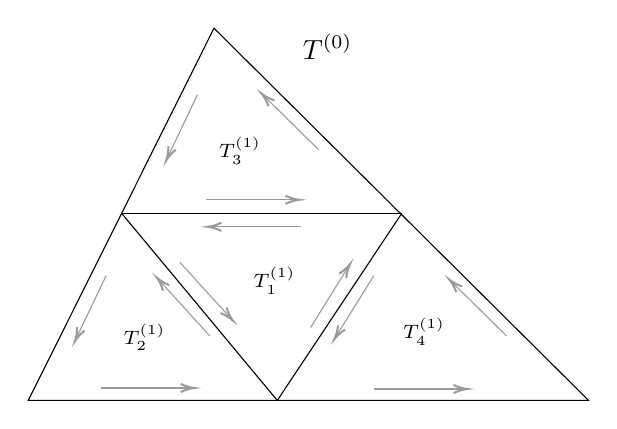
\begin{tikzpicture}[x=0.75pt,y=0.75pt,yscale=-1,xscale=1]
		%uncomment if require: \path (0,300); %set diagram left start at 0, and has height of 300
		
		%Shape: Triangle [id:dp22929948430382896] 
		\draw   (199.5,70.67) -- (380,250) -- (110,250) -- cycle ;
		%Straight Lines [id:da244981817401549] 
		\draw    (155,159.83) -- (290,159.83) ;
		%Straight Lines [id:da07991899539465663] 
		\draw    (155,159.83) -- (230,250) ;
		%Straight Lines [id:da21358766614612867] 
		\draw    (290,159.83) -- (230,250) ;
		%Straight Lines [id:da6197653203930451] 
		\draw [color={rgb, 255:red, 155; green, 155; blue, 155 }  ,draw opacity=1 ]   (195.5,153.32) -- (238.5,153.32) ;
		\draw [shift={(240.5,153.32)}, rotate = 180] [color={rgb, 255:red, 155; green, 155; blue, 155 }  ,draw opacity=1 ][line width=0.75]    (6.56,-1.97) .. controls (4.17,-0.84) and (1.99,-0.18) .. (0,0) .. controls (1.99,0.18) and (4.17,0.84) .. (6.56,1.97)   ;
		%Straight Lines [id:da5794917403292845] 
		\draw [color={rgb, 255:red, 155; green, 155; blue, 155 }  ,draw opacity=1 ]   (250,129.28) -- (223.93,103.63) ;
		\draw [shift={(222.5,102.23)}, rotate = 44.53] [color={rgb, 255:red, 155; green, 155; blue, 155 }  ,draw opacity=1 ][line width=0.75]    (6.56,-1.97) .. controls (4.17,-0.84) and (1.99,-0.18) .. (0,0) .. controls (1.99,0.18) and (4.17,0.84) .. (6.56,1.97)   ;
		%Straight Lines [id:da14151133839867325] 
		\draw [color={rgb, 255:red, 155; green, 155; blue, 155 }  ,draw opacity=1 ]   (191.5,102.73) -- (177.36,132.48) ;
		\draw [shift={(176.5,134.28)}, rotate = 295.42] [color={rgb, 255:red, 155; green, 155; blue, 155 }  ,draw opacity=1 ][line width=0.75]    (6.56,-1.97) .. controls (4.17,-0.84) and (1.99,-0.18) .. (0,0) .. controls (1.99,0.18) and (4.17,0.84) .. (6.56,1.97)   ;
		%Straight Lines [id:da6438773878089432] 
		\draw [color={rgb, 255:red, 155; green, 155; blue, 155 }  ,draw opacity=1 ]   (147.5,189.89) -- (133.36,219.64) ;
		\draw [shift={(132.5,221.45)}, rotate = 295.42] [color={rgb, 255:red, 155; green, 155; blue, 155 }  ,draw opacity=1 ][line width=0.75]    (6.56,-1.97) .. controls (4.17,-0.84) and (1.99,-0.18) .. (0,0) .. controls (1.99,0.18) and (4.17,0.84) .. (6.56,1.97)   ;
		%Straight Lines [id:da5035255329161727] 
		\draw [color={rgb, 255:red, 155; green, 155; blue, 155 }  ,draw opacity=1 ]   (145,243.99) -- (188,243.99) ;
		\draw [shift={(190,243.99)}, rotate = 180] [color={rgb, 255:red, 155; green, 155; blue, 155 }  ,draw opacity=1 ][line width=0.75]    (6.56,-1.97) .. controls (4.17,-0.84) and (1.99,-0.18) .. (0,0) .. controls (1.99,0.18) and (4.17,0.84) .. (6.56,1.97)   ;
		%Straight Lines [id:da20703213743187354] 
		\draw [color={rgb, 255:red, 155; green, 155; blue, 155 }  ,draw opacity=1 ]   (197.5,218.94) -- (173.35,192.37) ;
		\draw [shift={(172,190.89)}, rotate = 47.73] [color={rgb, 255:red, 155; green, 155; blue, 155 }  ,draw opacity=1 ][line width=0.75]    (6.56,-1.97) .. controls (4.17,-0.84) and (1.99,-0.18) .. (0,0) .. controls (1.99,0.18) and (4.17,0.84) .. (6.56,1.97)   ;
		%Straight Lines [id:da8174786530331881] 
		\draw [color={rgb, 255:red, 155; green, 155; blue, 155 }  ,draw opacity=1 ]   (340.5,218.94) -- (314.43,193.29) ;
		\draw [shift={(313,191.89)}, rotate = 44.53] [color={rgb, 255:red, 155; green, 155; blue, 155 }  ,draw opacity=1 ][line width=0.75]    (6.56,-1.97) .. controls (4.17,-0.84) and (1.99,-0.18) .. (0,0) .. controls (1.99,0.18) and (4.17,0.84) .. (6.56,1.97)   ;
		%Straight Lines [id:da7674415762467801] 
		\draw [color={rgb, 255:red, 155; green, 155; blue, 155 }  ,draw opacity=1 ]   (276.5,244.49) -- (319.5,244.49) ;
		\draw [shift={(321.5,244.49)}, rotate = 180] [color={rgb, 255:red, 155; green, 155; blue, 155 }  ,draw opacity=1 ][line width=0.75]    (6.56,-1.97) .. controls (4.17,-0.84) and (1.99,-0.18) .. (0,0) .. controls (1.99,0.18) and (4.17,0.84) .. (6.56,1.97)   ;
		%Straight Lines [id:da06674836216123325] 
		\draw [color={rgb, 255:red, 155; green, 155; blue, 155 }  ,draw opacity=1 ]   (276.5,189.89) -- (258.56,218.75) ;
		\draw [shift={(257.5,220.45)}, rotate = 301.87] [color={rgb, 255:red, 155; green, 155; blue, 155 }  ,draw opacity=1 ][line width=0.75]    (6.56,-1.97) .. controls (4.17,-0.84) and (1.99,-0.18) .. (0,0) .. controls (1.99,0.18) and (4.17,0.84) .. (6.56,1.97)   ;
		%Straight Lines [id:da5880950101661566] 
		\draw [color={rgb, 255:red, 155; green, 155; blue, 155 }  ,draw opacity=1 ]   (198.5,166.34) -- (241.5,166.34) ;
		\draw [shift={(196.5,166.34)}, rotate = 0] [color={rgb, 255:red, 155; green, 155; blue, 155 }  ,draw opacity=1 ][line width=0.75]    (6.56,-1.97) .. controls (4.17,-0.84) and (1.99,-0.18) .. (0,0) .. controls (1.99,0.18) and (4.17,0.84) .. (6.56,1.97)   ;
		%Straight Lines [id:da10416251901852114] 
		\draw [color={rgb, 255:red, 155; green, 155; blue, 155 }  ,draw opacity=1 ]   (207.15,209.95) -- (183,183.38) ;
		\draw [shift={(208.5,211.43)}, rotate = 227.73] [color={rgb, 255:red, 155; green, 155; blue, 155 }  ,draw opacity=1 ][line width=0.75]    (6.56,-1.97) .. controls (4.17,-0.84) and (1.99,-0.18) .. (0,0) .. controls (1.99,0.18) and (4.17,0.84) .. (6.56,1.97)   ;
		%Straight Lines [id:da2685827787461035] 
		\draw [color={rgb, 255:red, 155; green, 155; blue, 155 }  ,draw opacity=1 ]   (263.94,186.08) -- (246,214.93) ;
		\draw [shift={(265,184.38)}, rotate = 121.87] [color={rgb, 255:red, 155; green, 155; blue, 155 }  ,draw opacity=1 ][line width=0.75]    (6.56,-1.97) .. controls (4.17,-0.84) and (1.99,-0.18) .. (0,0) .. controls (1.99,0.18) and (4.17,0.84) .. (6.56,1.97)   ;
		
		% Text Node
		\draw (217.33,184.4) node [anchor=north west][inner sep=0.75pt]  [font=\scriptsize]  {$T_{1}^{( 1)}$};
		% Text Node
		\draw (154.67,211.73) node [anchor=north west][inner sep=0.75pt]  [font=\scriptsize]  {$T_{2}^{( 1)}$};
		% Text Node
		\draw (200.67,121.73) node [anchor=north west][inner sep=0.75pt]  [font=\scriptsize]  {$T_{3}^{( 1)}$};
		% Text Node
		\draw (289.33,209.07) node [anchor=north west][inner sep=0.75pt]  [font=\scriptsize]  {$T_{4}^{( 1)}$};
		% Text Node
		\draw (241,72.4) node [anchor=north west][inner sep=0.75pt]    {$T^{( 0)}$};
		
		
	\end{tikzpicture}
\end{figure}
	Starting with the triangle $ T^(0) $, we connect the mid-points of the edges and then we will get four \emph{congruent} triangles. By a simple geometrical argument we can see that the radius and the diameter of the triangles $ T^(1)_j $ for $ j=1,2,3,4 $ is half of the radius and perimeter of the original triangles. I.e. By doing the same process we will get smaller and smaller triangles at each step and at step $ n $ we have
	\[ d^(n) = 2^{-n} d^{(0)}, \qquad p^{n} = 2^{-n}p^{(0)}. \]
	
	{\color{red} \noindent TODO: TO BE WRITTEN}
	
\end{proof}



\section{Solved Problems}

\begin{problem}[From Stein]
	Suppose $ f $ is continuously complex differentiable on $ \Omega $, and $ T\subset\Omega $ is a triangle whose interior is also contained in $ \Omega $. Apply Green's theorem to show that
	\[ \int_T f(z)dz = 0. \]
	This provides a proof of Goursat's theorem under the additional assumption that $ f' $ is continuous. \emph{Hint: Green's theorem says that if $ (F,G) $ is a continuously differentiable vector field, then}
	\[ \int_T Fdx + Gdy = \int_{int(T)} \left( \frac{\partial G}{\partial x} - \frac{\partial F}{\partial y} \right) dx dy. \]
	\emph{For appropriate $ F $ and $ G $, one can then use the Cauchy-Riemann equations.}
\end{problem}
\begin{solution}
	Let $ T $ be parameterized by piece-wise smooth $ \gamma:[0,1] \to \R $, given by $ \gamma(t) = x(t) + iy(t) $. Let $ f = u+iv $. By the definition of the Contour integral
	\begin{align*}
		\int_T f(z)dz &= \int_{a}^{b} f(\gamma(t))\gamma'(t)dt = \int_{a}^{b} (u(x,y)+iv(x,y)) (x'(t)+iy'(t)) dt \\
		&=\int_{a}^{b}((u+iv)x'(t) + (iu-v)y'(t)) dt = \int_T f dx + g dy,
	\end{align*}
	where
	\[ f(u,v) = u+iv, \qquad g(u,v) = iu-v. \]
	Using Green's theorem
	\[ \int_T fdx+gdy = \int_{T^\circ} \left( \frac{\partial g}{\partial x} - \frac{\partial f}{\partial y} \right) dx dy  \]
	where $ T^\circ $ denotes the interior of the triangle. Observe that
	\[ \frac{\partial f}{\partial y} = u_y + i v_y,\qquad \frac{\partial g}{\partial x}=iu_x - v_x. \]
	Thus
	\[ \frac{\partial g}{\partial x} - \frac{\partial f}{\partial y} = - (u_y + v_x) + (u_x - v_y) = 0, \]
	where we have used the fact that the Cauchy-Riemann equations hold (as $ f $ is complex differentiable.)
	Thus
	\[ \int_T f(z) dz = 0. \]
\end{solution}

\begin{observation}
	In the question above, using the fact that $ f $ is complex differentiable, \emph{plus} the extra regularity condition, that $ f' $ is continuous, we can simply use the Green's theorem to prove a variant of the Goursat's theorem. The reason that we need the extra regularity is that for the Green's theorem, we need the partial derivatives of the components of the vector field to be continuous.
\end{observation}


\begin{problem}[From Stein]
	Let $ \Omega $ be an open subset of $ C $ and let $ T\subset \Omega $ be a triangle whose interior is also contained in $ \Omega $. Suppose that $ f $ is a function holomorphic in $ \Omega $ except possibly at a point $ \omega \in T^\circ $, where $ T^\circ $ is the interior of the triangle. Prove that if $ f $ is bounded near $ w $, then
	\[ \int_T f(z)dz  = 0. \]
\end{problem}
\begin{solution}
	Consider the following figure
	\begin{figure}[h!]
	\centering
	
	
	\tikzset{every picture/.style={line width=0.75pt}} %set default line width to 0.75pt        
	
	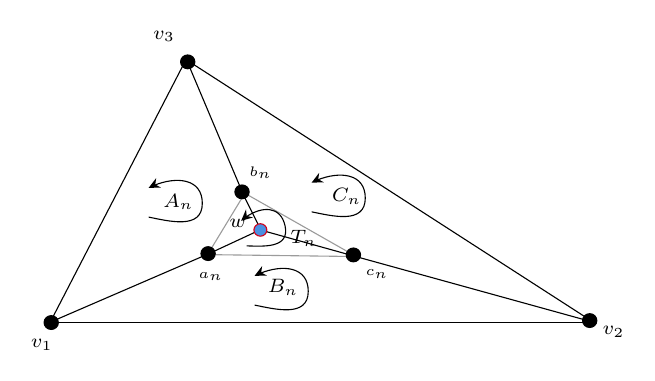
\begin{tikzpicture}[x=0.75pt,y=0.75pt,yscale=-1,xscale=1]
		%uncomment if require: \path (0,300); %set diagram left start at 0, and has height of 300
		
		%Straight Lines [id:da5441237327441648] 
		\draw    (388.08,204.69) -- (273.58,173.05) -- (227.61,160.24) ;
		%Straight Lines [id:da06891301104748981] 
		\draw    (228.43,159.77) -- (203.24,171.47) -- (126.36,204.69) ;
		%Straight Lines [id:da59311535047521] 
		\draw    (192.12,78.46) -- (219.6,143.63) -- (228.1,160.72) ;
		%Straight Lines [id:da6544515968635645] 
		\draw    (191.79,78.15) -- (126.36,204.69) ;
		%Straight Lines [id:da10139955539512191] 
		\draw    (388.08,204.69) -- (126.36,204.69) ;
		%Straight Lines [id:da8917816158697542] 
		\draw    (388.08,204.69) -- (191.79,78.15) ;
		%Shape: Ellipse [id:dp8443162743719417] 
		\draw  [color={rgb, 255:red, 208; green, 2; blue, 27 }  ,draw opacity=1 ][fill={rgb, 255:red, 74; green, 144; blue, 226 }  ,fill opacity=1 ] (224.5,160.24) .. controls (224.5,158.58) and (225.9,157.24) .. (227.61,157.24) .. controls (229.33,157.24) and (230.72,158.58) .. (230.72,160.24) .. controls (230.72,161.9) and (229.33,163.25) .. (227.61,163.25) .. controls (225.9,163.25) and (224.5,161.9) .. (224.5,160.24) -- cycle ;
		%Straight Lines [id:da25333294259616235] 
		\draw [color={rgb, 255:red, 155; green, 155; blue, 155 }  ,draw opacity=1 ]   (220.25,142.37) -- (202.58,171.47) ;
		%Straight Lines [id:da20450070698173506] 
		\draw [color={rgb, 255:red, 155; green, 155; blue, 155 }  ,draw opacity=1 ]   (273.58,173.05) -- (201.28,172.11) ;
		%Straight Lines [id:da03358532217874943] 
		\draw [color={rgb, 255:red, 155; green, 155; blue, 155 }  ,draw opacity=1 ]   (273.25,172.74) -- (220.91,143) ;
		%Shape: Boxed Bezier Curve [id:dp3812843843820022] 
		\draw    (221,167.92) .. controls (228.54,168.05) and (241.94,169.42) .. (239.52,158.29) .. controls (237.32,148.22) and (228.03,148.87) .. (220.62,154.05) ;
		\draw [shift={(218.36,155.82)}, rotate = 318.79] [fill={rgb, 255:red, 0; green, 0; blue, 0 }  ][line width=0.08]  [draw opacity=0] (5.36,-2.57) -- (0,0) -- (5.36,2.57) -- (3.56,0) -- cycle    ;
		%Shape: Boxed Bezier Curve [id:dp1762642951465938] 
		\draw    (224.83,196.44) .. controls (234.25,198.27) and (250.68,202.78) .. (250.68,189.82) .. controls (250.68,177.83) and (238.33,176.69) .. (227.44,181.16) ;
		\draw [shift={(224.83,182.35)}, rotate = 333.17] [fill={rgb, 255:red, 0; green, 0; blue, 0 }  ][line width=0.08]  [draw opacity=0] (5.36,-2.57) -- (0,0) -- (5.36,2.57) -- (3.56,0) -- cycle    ;
		%Shape: Boxed Bezier Curve [id:dp4474810905143487] 
		\draw    (252.31,151.52) .. controls (261.73,153.35) and (278.16,157.86) .. (278.16,144.89) .. controls (278.16,132.9) and (265.81,131.76) .. (254.92,136.23) ;
		\draw [shift={(252.31,137.43)}, rotate = 333.17] [fill={rgb, 255:red, 0; green, 0; blue, 0 }  ][line width=0.08]  [draw opacity=0] (5.36,-2.57) -- (0,0) -- (5.36,2.57) -- (3.56,0) -- cycle    ;
		%Shape: Boxed Bezier Curve [id:dp07272842875956065] 
		\draw    (173.79,154.05) .. controls (183.21,155.88) and (199.64,160.39) .. (199.64,147.43) .. controls (199.64,135.44) and (187.3,134.29) .. (176.41,138.76) ;
		\draw [shift={(173.79,139.96)}, rotate = 333.17] [fill={rgb, 255:red, 0; green, 0; blue, 0 }  ][line width=0.08]  [draw opacity=0] (5.36,-2.57) -- (0,0) -- (5.36,2.57) -- (3.56,0) -- cycle    ;
		%Shape: Ellipse [id:dp033053623020744105] 
		\draw  [fill={rgb, 255:red, 0; green, 0; blue, 0 }  ,fill opacity=1 ] (189.17,79.25) .. controls (189.17,77.42) and (190.71,75.93) .. (192.61,75.93) .. controls (194.5,75.93) and (196.04,77.42) .. (196.04,79.25) .. controls (196.04,81.09) and (194.5,82.57) .. (192.61,82.57) .. controls (190.71,82.57) and (189.17,81.09) .. (189.17,79.25) -- cycle ;
		%Shape: Ellipse [id:dp6784778105513676] 
		\draw  [fill={rgb, 255:red, 0; green, 0; blue, 0 }  ,fill opacity=1 ] (123.41,204.85) .. controls (123.41,203.01) and (124.95,201.53) .. (126.85,201.53) .. controls (128.75,201.53) and (130.28,203.01) .. (130.28,204.85) .. controls (130.28,206.68) and (128.75,208.17) .. (126.85,208.17) .. controls (124.95,208.17) and (123.41,206.68) .. (123.41,204.85) -- cycle ;
		%Shape: Ellipse [id:dp36701946193477464] 
		\draw  [fill={rgb, 255:red, 0; green, 0; blue, 0 }  ,fill opacity=1 ] (382.85,203.9) .. controls (382.85,202.07) and (384.38,200.58) .. (386.28,200.58) .. controls (388.18,200.58) and (389.72,202.07) .. (389.72,203.9) .. controls (389.72,205.73) and (388.18,207.22) .. (386.28,207.22) .. controls (384.38,207.22) and (382.85,205.73) .. (382.85,203.9) -- cycle ;
		%Shape: Ellipse [id:dp1796206915353047] 
		\draw  [fill={rgb, 255:red, 0; green, 0; blue, 0 }  ,fill opacity=1 ] (198.99,171.63) .. controls (198.99,169.8) and (200.52,168.31) .. (202.42,168.31) .. controls (204.32,168.31) and (205.86,169.8) .. (205.86,171.63) .. controls (205.86,173.47) and (204.32,174.95) .. (202.42,174.95) .. controls (200.52,174.95) and (198.99,173.47) .. (198.99,171.63) -- cycle ;
		%Shape: Ellipse [id:dp5441347681687478] 
		\draw  [fill={rgb, 255:red, 0; green, 0; blue, 0 }  ,fill opacity=1 ] (215.34,141.89) .. controls (215.34,140.06) and (216.88,138.57) .. (218.78,138.57) .. controls (220.68,138.57) and (222.21,140.06) .. (222.21,141.89) .. controls (222.21,143.73) and (220.68,145.21) .. (218.78,145.21) .. controls (216.88,145.21) and (215.34,143.73) .. (215.34,141.89) -- cycle ;
		%Shape: Ellipse [id:dp8872658534774043] 
		\draw  [fill={rgb, 255:red, 0; green, 0; blue, 0 }  ,fill opacity=1 ] (269,172.26) .. controls (269,170.43) and (270.53,168.94) .. (272.43,168.94) .. controls (274.33,168.94) and (275.87,170.43) .. (275.87,172.26) .. controls (275.87,174.1) and (274.33,175.59) .. (272.43,175.59) .. controls (270.53,175.59) and (269,174.1) .. (269,172.26) -- cycle ;
		
		% Text Node
		\draw (115.77,211.75) node [anchor=north west][inner sep=0.75pt]  [font=\scriptsize]  {$v_{1}$};
		% Text Node
		\draw (174.66,63.05) node [anchor=north west][inner sep=0.75pt]  [font=\scriptsize]  {$v_{3}$};
		% Text Node
		\draw (391.23,205.42) node [anchor=north west][inner sep=0.75pt]  [font=\scriptsize]  {$v_{2}$};
		% Text Node
		\draw (196.58,179.29) node [anchor=north west][inner sep=0.75pt]  [font=\tiny]  {$a_{n}$};
		% Text Node
		\draw (221.05,128.37) node [anchor=north west][inner sep=0.75pt]  [font=\tiny]  {$b_{n}$};
		% Text Node
		\draw (277.06,178.02) node [anchor=north west][inner sep=0.75pt]  [font=\tiny]  {$c_{n}$};
		% Text Node
		\draw (211.37,153.75) node [anchor=north west][inner sep=0.75pt]  [font=\scriptsize]  {$w$};
		% Text Node
		\draw (179.6,141.6) node [anchor=north west][inner sep=0.75pt]  [font=\scriptsize]  {$A_{n}$};
		% Text Node
		\draw (230,182.8) node [anchor=north west][inner sep=0.75pt]  [font=\scriptsize]  {$B_{n}$};
		% Text Node
		\draw (260.8,138.8) node [anchor=north west][inner sep=0.75pt]  [font=\scriptsize]  {$C_{n}$};
		% Text Node
		\draw (240.8,159.2) node [anchor=north west][inner sep=0.75pt]  [font=\scriptsize]  {$T_{n}$};
		
		
	\end{tikzpicture}
\end{figure}
	where we connect the point $ w \in T^\circ $ to the edges. On each of the line segments $ (v_i,w) $  we choose the points $ a_n,b_n,c_n $ respectively for $ i=1,2,3 $ such that $ a_n,b_n,c_n \to w $ as $ n \to \infty $. By the cancellation of the integral on the paths that have been traversed twice on opposite directions we can write
	\[ \int_{T}f(z)dz = \int_{A_n} f(z)dz + \int_{B_n}f(z)dz + \int_{C_n}f(z)dz + \int_{T_n}f(z)dz,  \]
	were $ A_n,B_n, $ and $ C_n $ are the tetragons as shown above, and $ T_n $ is the central triangle. Observe that the integration over each tetragon can further be broken down into two integral on two triangles, where by applying the Goursat's theorem it evaluates to zero. Thus the only remaining term will be
	\[ \int_{T} f(z)dz = \int_{T_n}f(z)dz. \]
	We can write
	\[ \abs{\int_{T} f(z)dz} = \abs{\int_{T_n}f(z)dz} \leq \max_{z\in T_n}\abs{f(z)} \ell(T_n). \]
	Since the function $ f $ is bounded around $ w $ then $ \max_{z\in T_n}\abs{f(z)} \leq C $ for some $ C\in \R $ and $ \ell(T_n)\to 0 $ as $ n\to\infty $, we will have
	\[ \int_T f(z) dz = 0. \]
\end{solution}


\begin{problem}[From Stein]
	Suppose $ f:\D \to \C $ is holomorphic. Show that the diameter $ d=\sup_{z,w\in\D}\abs{f(z)-f(w)} $ of the image of $ f $ satisfies
	\[ 2\abs{f'(0)} \leq d. \]
	Moreover, it can be show that the equality holds precisely when $ f $ is linear, $ f(z) = a_0 + a_1 z $. \emph{Hint: You can use the fact that $ 2f'(0) = \frac{1}{2\pi i}\int_{\abs{\xi}=r}\frac{f(\xi)-f(-\xi)}{\xi^2}d\xi $ whenever $ 0<r<1 $.}
\end{problem}
\begin{solution}
	Using the Cauchy integral formula we can write
	\[ f'(0) = \frac{1}{2\pi i}\int_{\abs{\xi}=r} \frac{f(\xi)}{\xi^2}d\xi = - \int_{\abs{\xi}=r} \frac{f(-\xi)}{\xi^2}d\xi, \]
	where the second equality holds by a simple change of variable. Then we can write
	\[ 2f'(0) = \frac{1}{2\pi i}\int_{\abs{\xi}=r}\frac{f(\xi)-f(-\xi)}{\xi^2} d\xi. \] 
	Then
	\begin{align*}
		2\abs{f'(0)} &= \frac{1}{2\pi i}\abs{\int_{\abs{\xi}=r}\frac{f(\xi)-f(-\xi)}{\xi^2} d\xi} \\
		&\leq \frac{1}{2\pi i}\int_{\abs{\xi}=r}\frac{\abs{f(\xi)-f(-\xi)}}{\abs{\xi^2}} d\xi\\
		&\leq \frac{d}{2\pi} \int_{\abs{\xi}=r}\frac{1}{\abs{\xi}^2}d\xi \\
		&\leq \frac{d}{2\pi} \frac{2\pi r}{r^2} = d/r. 
	\end{align*}
	This for all $ r \in (0,1) $ we have $ 2\abs{f'(0)}\leq d/r $. This implies
	\[ 2\abs{f'(0)}\leq \inf_{r\in(0,1)}\frac{d}{r} = d. \]
\end{solution}

\begin{problem}[From Stein]
	If $ f $ is holomorphic function on the strip $ -1<y<1 $ and $ x\in \R $ with
	\[ \abs{f(z)}\leq A(1+\abs{z})^\eta,\qquad \text{$ \eta $ a fixed real number} \]
	for all $ z $ in that strip, show that for each integer $ n\geq 0 $ there exists $ A_n\geq 0 $ so that 
	\[ \abs{f^{(n)}(x)}\leq A_n(1+\abs{x})^\eta, \qquad \text{for all $ x\in\R $}. \]
	\emph{Hint: Use the Cauchy inequalities.}
\end{problem}
\begin{solution}
	Let $ x\in \R $. This point is in the strip where $ f $ is holomorphic. Consider the set $ \abs{z-x}=R $ that is a circle with radius $ R $ centered at $ x $. Then So using the Cauchy inequalities
	\[ \abs{f^{(n)}(x)}\leq \frac{n!}{R^n}\sup_{\abs{z-x}=r} \abs{f(z)} \leq \frac{An!}{R^n} \sup_{\abs{z-x}=r}(1+\abs{z})^\eta \leq \frac{An!}{R^n}(1+\abs{x+R})^\eta\leq \frac{An!}{R^n}(1+\abs{x}+R)^\eta.  \]
	By letting $ R=1/2 $ and using the fact that $ 3/2+\abs{x}\leq 3/2(1+\abs{x}) $, we will get
	\[ \abs{f^{(n)}(x)} \leq \frac{An!}{(1/2)^n}\cdot(\frac{3}{2})^\eta (1+\abs{x})^\eta = A_n (1+\abs{x})^\eta \]
\end{solution}

\end{document}